\documentclass{polyu-comp}
\usepackage[T1]{fontenc}
\usepackage{tabularx} % For tables with adjustable columns
\usepackage{url}
\usepackage{booktabs}
\usepackage{graphicx}
\usepackage{algorithm}
\usepackage{algorithmic}
\usepackage{tikz}
\usetikzlibrary{shapes.geometric, arrows.meta, positioning, fit, calc}
\usepackage[absolute]{textpos}
\usepackage{listings}
\usepackage{amssymb}
\usepackage{amsmath}
\usepackage{titlesec}
\usepackage[table]{xcolor} % 用于表格行背景色
\usepackage{pgfplots}
\pgfplotsset{compat=1.18} % 确保使用最新的绘图兼容模式
\newcolumntype{Y}{>{\centering\arraybackslash}X}
\newcommand{\sectionbreak}{\clearpage}

\lstset{
    basicstyle=\ttfamily\small,      % 代码字体
    numbers=left,                    % 行号显示在左侧
    numberstyle=\tiny\color{gray},   % 行号样式
    stepnumber=1,                    % 行号间隔
    numbersep=5pt,                   % 行号与代码的距离
    backgroundcolor=\color{white},   % 背景色
    showspaces=false,                % 不显示空格符号
    showstringspaces=false,          % 字符串中不显示空格符号
    showtabs=false,                  % 不显示制表符
    frame=single,                    % 给代码加边框
    rulecolor=\color{black},         % 边框颜色
    tabsize=2,                       % 制表符宽度
    captionpos=b,                    % 标题位置（底部）
    breaklines=true,                 % 自动换行
    breakatwhitespace=false,         % 
    title=\lstname,                  % 
    keywordstyle=\color{blue},       % 关键字颜色
    commentstyle=\color{green!50!black}, % 注释颜色
    stringstyle=\color{red},         % 字符串颜色
    escapeinside={\%*}{*)},          % 如果需要在代码中写 LaTeX
    morekeywords={*,...}             % 如果需要添加额外的关键字
}

% Cover fields (override if needed)
\renewcommand{\CompTitle}{Compress-Transfer-Decompress for LLM Serving: cuSZp-Enabled CPU--GPU Data Pipeline in vLLM}
\renewcommand{\CompStudentName}{KONG Zirui}
\renewcommand{\CompStudentID}{22103493D}
\renewcommand{\CompStudentSupervisor}{Dr ZHANG Zhaorui}
\renewcommand{\CompStreamCode}{61435-FCS}
\renewcommand{\CompCoExaminer}{Prof. WU Yujie}
\renewcommand{\CompAssessor}{Prof. YANG Hongxia}
\renewcommand{\CompSubmissionDate}{10 April 2026}

\begin{document}

% Cover page
\printCompCover

% Abstract
\clearpage
\section*{Abstract}
\addcontentsline{toc}{section}{Abstract}
As context windows in Large Language Models (LLMs) expand, the Key-Value (KV) cache consumes massive amounts of memory during inference, which creates a severe bottleneck. When GPU VRAM runs out, serving engines like vLLM will avoid crashes by swapping inactive KV cache blocks to the host CPU. However, sending all this data back and forth across the PCIe bus will create a huge time latency, which slows down the entire inference process.

To address this bottleneck, this project introduces a ``Compress-Transfer-Decompress'' data pipeline integrated directly into vLLM. The approach uses cuSZp, a fast lossy compression framework that runs on the local GPU. A custom C++ wrapper uses PyBind11 to connect the underlying CUDA APIs to vLLM's Python CacheEngine. Instead of modifying the core engine code, the Monkey-Patching technique was used to intercept the KV cache tensors. The system compresses them before they hit the PCIe bus and decompresses them when the engine needs. This greatly reduces the physical payload.

The setup was tested on an NVIDIA RTX 5080 GPU. Instead of using dummy data, real Layer-0 key embeddings were extracted from eight different models, including Qwen2.5, GPT-2, and OPT. An error bound of $1 \times 10^{-4}$ was set to ensure the model generation quality remained safe. As the GPU handles compression so quickly, the time saved on PCIe transfer easily covers the computational overhead. Testing showed the effective Swap-Out bandwidth improved to 1.77$\times$, and Swap-In bandwidth improved to 2.08$\times$. The pipeline reduced the data from 2.42$\times$ to 3.06$\times$. This proves that compressing tensors at runtime is a practical method to bypass PCIe limitations in LLM services.


% Acknowledgements
\clearpage
\section*{Acknowledgments}
\addcontentsline{toc}{section}{Acknowledgments}

First of all, I would like to express my deepest gratitude to my supervisor, \textbf{Dr. ZHANG Zhaorui}, for her valuable guidance, continuous encouragement, and helpful suggestions throughout the research and development process of this project. Her expertise in systems and performance optimization provided the foundation for this work.

I am also sincerely grateful to \textbf{Prof. WU Yujie} and \textbf{Prof. YANG Hongxia} for their time in reviewing the thesis. Their professional suggestions have significantly enhanced the quality of this final report.

Special thanks to the Department of Computing at The Hong Kong Polytechnic University for providing essential research facilities and an engaging academic environment.

Personally, I want to thank my family and my beloved for their unwavering support and trust. Stepping out of my comfort zone in front-end development and AI/robotics research to study the complexities of CUDA-accelerated systems has been a challenging journey. Fortunately, having a better half who also studies computer science provided me with inspiration and comfort; her patience and encouragement were my greatest motivations.

Finally, as I prepare to start my Master's studies at The Chinese University of Hong Kong, I look back on my undergraduate years at PolyU with immense gratitude for the personal growth and opportunities I gained.


\tableofcontents

% List of Tables and Figures
\clearpage
\addcontentsline{toc}{section}{List of Tables}
\listoftables

\clearpage
\addcontentsline{toc}{section}{List of Figures}
\listoffigures

% 正文开始

\section{Introduction}

\subsection{Motivation}
In recent years, Large Language Models (LLMs) have demonstrated unprecedented capabilities \cite{10.1145/3744746} across a wide range of Natural Language Processing (NLP) tasks. With the increasing demand for analyzing and generating longer documents, modern LLMs are designed to support the massive length of context windows. However, this capability has a serious memory challenge during the autoregressive inference. In particular, the key value (KV) cache used to store the tensor of previous tokens to avoid redundant recalculation grows rapidly with the increase of sequence length and batch size. To accommodate requests that exceed the Video Random Access Memory (VRAM) capacity of Graphics Processing Units (GPUs), advanced service engines such as vLLM \cite{kwon2023efficient} adopt memory management techniques, such as PagedAttention, dynamically offloading inactive KV cache blocks to the host Central Processing Unit (CPU) memory and restoring them when needed. While highly effective in preventing Out-Of-Memory (OOM) failures, this offloading mechanism exposes a critical hardware limitation, long-context generation, which must be addressed to maintain high-throughput.

\subsection{Problem Statement}
The main bottleneck \cite{8763922} in KV cache swapping lies in the physical Peripheral Component Interconnect Express (PCIe) bus that connects the CPU and GPU. As PCIe bandwidth is several orders of magnitude lower than the High-Bandwidth Memory (HBM) inside the GPU, the transmission of a large number of uncompressed multidimensional tensor data between the GPU and the CPU memory will cause significant delays. This delay can substantially block the GPU computation pipeline and reduce the overall inference speed. Therefore, without optimizing the data transmission payload, PCIe bandwidth wall seriously limits the actual use effect of the KV cache.

\subsection{Project Objectives}
To ease the bottleneck of the above data transmission, this project aims to design a ``Compress-Transfer-Decompress'' data pipeline with vLLM. The specific objectives of this project are as follows:
\begin{itemize}
    \item \textbf{Accelerate KV Cache Swapping:} To reduce the amount of physical data transmitted through the PCIe bus by using lossy compression with error limits before transmission, and quickly decompress the data when it is returned to the GPU.
    \item \textbf{Seamless Integration into vLLM:} To successfully embed this compressed pipeline into the vLLM PagedAttention architecture to ensure compatibility and stability without interrupting the core memory management function.
\end{itemize}

\subsection{Key Contributions}
To fulfill these objectives, this project uses \textbf{cuSZp} \cite{huang2023cuszp}, a highly optimized, GPU-accelerated, and error-bounded lossy compression framework. The key contributions of this project are as follows:
\begin{itemize}
    \item \textbf{Custom PyBind11 \cite{RODRIGUEZ_LUZARDO_2022} Wrapper for cuSZp:} Designed and compiled a robust C++ wrapper via PyBind11, directly exposing the native cuSZp compression and decompression Application Programming Interfaces (APIs) to Python with minimal calls.
    \item \textbf{Implementation of Compressed Swap Logic in vLLM:} Developed an integration pipeline using Monkey-Patching \cite{Hunt2023} technique to intercept and override vLLM's native \texttt{swap\_in} and \texttt{swap\_out} tensor block operations with Compress-Transfer-Decompress mechanism.
    \item \textbf{Comprehensive Automated Benchmark Suite:} Created an automatic analysis pipeline that slices Layer-0 \cite{zhang-etal-2024-investigating} key embeddings to evaluate the system's performance. The solution has been basically verified in eight most advanced LLMs, including GPT-2 \cite{radford2019language}, Qwen2.5 \cite{qwen2.5}, OPT \cite{zhang2022optopenpretrainedtransformer}, Pythia \cite{biderman2023pythia}, and TinyLlama \cite{zhang2024tinyllama}.
\end{itemize}

\subsection{Thesis Organization}
The remainder of this thesis is structured as follows. \textbf{Section 2} reviews the background of LLM serving, memory bottlenecks, and the principles of error-bounded lossy tensor compression. \textbf{Section 3} introduces the methodology, including the latency trade-off model and the selection of the error bound. \textbf{Section 4} presents the system design and implementation details of the C++ wrapper and vLLM integration. \textbf{Section 5} outlines the experimental setup and evaluations of the benchmark results. \textbf{Section 6} discusses the interpretation of results, hardware utilization, and implementation challenges. \textbf{Section 7} summarizes the thesis and suggests directions for future work.


\section{Background and Literature Review}

\subsection{LLM Serving and the KV Cache}

\subsubsection{Autoregressive Generation and the KV Cache}
LLMs based on transformer architecture generally generate text in an autoregressive manner. This means that predicting the next token requires the model to process all preceding tokens in the sequence. During inference, especially the decoding stage, calculating the attention of a new token requires the K and V tensors of all previously generated tokens. Recomputing these tensors at every generation step is infeasible. To optimize it, the inference engine uses a mechanism called KV caching. By storing the K and V tensors in memory after the first computation, the model can reuse them in subsequent steps to achieve significant computational acceleration at the cost of memory capacity. However, as the length of the context windows and batch sizes increase, the occupied space of the KV cache grows rapidly, and it quickly becomes a main memory consumer during inference.

\subsubsection{vLLM and PagedAttention}
To manage the massive memory requirements of the KV Cache, \textbf{vLLM} introduced PagedAttention, which will partition the continuous KV Cache into fixed-size and non-contiguous blocks. When the GPU VRAM is exhausted due to incoming requests or long sequence generation, vLLM's \texttt{CacheEngine} automatically intervenes. It frees up VRAM by preempting lower-priority requests and offloading (swapping out) their associated KV blocks to the host CPU RAM. Once the GPU has sufficient resources to resume the preempted request, the \texttt{CacheEngine} restores (swaps in) the blocks to VRAM. While this swapping mechanism prevents OOM errors, it introduces severe latency overhead that depends on the hardware's data transmission rate.

\subsection{Memory Bottlenecks in GPU Computing}
In modern heterogeneous computing systems, the performance of data-intensive operations largely depends on memory bandwidth. There is a significant difference between the internal bandwidth of the GPU and the interconnect bandwidth that connects the GPU to the host CPU:
\begin{itemize}
    \item \textbf{GPU VRAM Bandwidth:} High-end GPUs are equipped with High Bandwidth Memory (HBM) or ultra-fast GDDR memory (e.g., GDDR7 on the RTX 5080), capable of internal data transmission rates exceeding $1,000\text{ GB/s}$.
    \item \textbf{CPU-GPU PCIe Bandwidth:} In contrast, data transmission between the host CPU memory and GPU VRAM must traverse the Peripheral Component Interconnect Express (PCIe) bus. Even with a modern PCIe Gen 4.0 or Gen 5.0 connection, the theoretical bandwidth is limited between $32\text{ GB/s}$ and $64\text{ GB/s}$, and the actual effective bandwidth is usually much lower.
\end{itemize}
During the loading and offloading of KV caches in vLLM, uncompressed Gigabyte tensor data will pass through this narrow PCIe channel. These bandwidth limitations create a ``Memory Wall'' \cite{10.1145/3458817.3476205} where the GPU is waiting for data from the CPU, severely limiting the overall inference speed of LLMs.

\subsection{Data Compression for Tensors}
To alleviate the PCIe bandwidth bottleneck, data compression can be applied to reduce the data payload before transmission. Compression technologies are usually divided into two categories.

\subsubsection{Lossless and Lossy Compression}
\textbf{Lossless Compression} algorithms \cite{alma991085870187406532} guarantee bit-by-bit reconstruction of the original data. However, the floating-point tensors generated by neural networks are full of random noise in their final decimal places. As these trailing digits fluctuate constantly, the lossless compression algorithms cannot find the repeating patterns, resulting in low compression ratios (often under 1.5$\times$). As a result, lossless methods cannot shrink the data enough to speed up the PCIe transmission.

\textbf{Lossy Compression} \cite{9380370} achieves a significantly higher compression ratio by discarding less important information. Although this may introduce noise or precision loss, the neural network is inherently robust to small perturbations in the activation process. The challenge of traditional lossy algorithms is that unpredictable data loss will slowly affect the results through each layer of LLM, resulting in a significant decline in output quality (e.g., hallucination).

\subsubsection{Error-Bounded Lossy Compression}
To balance high compression ratios and high quality, Error-Bounded Lossy Compression frameworks have been developed. These algorithms allow developers to define mathematical error boundaries, guaranteeing that the difference between the raw data point ($x_i$) and the decompressed data point ($x'_i$) will never exceed the predefined threshold $\epsilon$ (i.e., $|x_i - x'_i| \leq \epsilon$). This high-precision control ensures that the accuracy of the KV cache is kept within a safe range while reducing the incoming tensor data.

\subsection{Introduction to cuSZp}
In this project, the \textbf{cuSZp} framework was used as the underlying compression engine. cuSZp is a fast lossy compression program with error bounds, which is specially designed for floating-point data. There are several reasons for using it:
\begin{itemize}
    \item \textbf{GPU-Accelerated Parallel Computation:} Unlike CPU-based compressors, cuSZp is implemented in Compute Unified Device Architecture (CUDA), allowing it to use thousands of GPU cores. This parallel operation ensures that the time spent compressing data will not exceed the time saved during PCIe transmission.
    \item \textbf{High Throughput:} cuSZp focuses on high-speed encoding and decoding rather than emphasizing maximal compression ratios. This concept can directly reduce the data transmission delay in LLM calculations.
    \item \textbf{Precise Error Control:} cuSZp will strictly follow the user-defined absolute or relative error limits to ensure the integrity of the KV cache and maintain the generation quality of LLMs.
\end{itemize}


\section{Methodology}
\label{sec:methodology}

This section introduces the details of the system architecture and implementation strategy of integrating the cuSZp lossy compression program into the vLLM inference engine. This integration aims to alleviate the PCIe bandwidth bottleneck while maintaining structural compatibility with the existing memory management of vLLM

\subsection{System Integration Strategy}
This integration is implemented without modifying the vLLM source code. Instead, a Monkey-Patching technique was used to intercept \texttt{CacheEngine} mechanisms of vLLM. Specifically, the default methods \texttt{\_swap\_out\_blocks\_to\_host} and \texttt{\_swap\_in\_blocks\_from\_host} in the \texttt{vllm.worker.cache\_engine} module are replaced with the new functions that handle the compression logic at runtime via a special \texttt{CompressedCacheEngineMonkeyPatch} class. The underlying C++ cuSZp API was linked directly to Python using PyBind11. To standardize the data, the \texttt{CuSZpCompressor} module transforms all incoming tensors into flattened 1-Dimension (1-D) arrays of single-precision floats. 

Another critical challenge addressed in this integration is synchronization. Typically, using a custom CUDA kernel within PyTorch \cite{NEURIPS2019_bdbca288} will cause a pause to wait for synchronization. When the compression program runs on different channels, the GPU needs frequent pauses to synchronize data streams, resulting in serious pipeline congestion. To solve this, the wrapper of the program will directly extract the current PyTorch active CUDA stream with the \path{c10::cuda::getCurrentCUDAStream().stream()} API. All compression and decompression tasks were dispatched to this shared stream. This low-level trick completely avoids synchronization pauses. The customized compressor can queue the workload perfectly and synchronize with the PyTorch asynchronous operation of vLLM.

By the original design, vLLM's native \texttt{BlockSpaceManager} only handles fixed-size memory blocks. Since compressed data streams are variable in length, relying on the standard CPU cache allocation is not feasible. To work around this limitation, the system implements a separate Python dictionary named \texttt{compressed\_blocks\_store}. This dictionary is used as a custom tracking system. It indexes every compressed block on the CPU using a composite key, which means that the layer index is combined with the destination block index (\texttt{(layer\_idx, dst\_idx)}). Alongside the byte stream, the store also saves the metadata required for later decompression, specifically the original tensor size, structural shape, and the calculated absolute error bound (\texttt{actual\_eb}).

Additionally, a strict safety measure has been formulated. If a tensor block resists any compressions due to compression error, the system simply cancels the compression attempt. It then immediately falls back to the original vLLM routine (\texttt{\_swap\_out\_blocks\_to\_host\_original()}) to transfer the original and uncompressed payload safely.

\subsection{The Compress-Transfer-Decompress Method}
By overriding vLLM's memory operations, the system changes from a direct physical transfer model to a \textit{Compress-Transfer-Decompress} method to maximize PCIe throughput efficiency:

\begin{algorithm}[htbp]
\caption{Dynamic Error-Bounded Compressed Swap-Out Pipeline}
\label{alg:swap_out}
\begin{algorithmic}[1]
\REQUIRE Uncompressed KV tensor $T_{gpu}$, Relative Error Bound $\epsilon_{rel}$, Target CPU indices $(L_{idx}, D_{idx})$
\ENSURE Compressed bitstream $B_{cpu}$ stored in Host RAM with metadata
\STATE $R \gets \max(T_{gpu}) - \min(T_{gpu})$ \COMMENT{Calculate range via CUDA reduction}
\IF{$R < 10^{-6}$}
    \STATE $R \gets 10^{-6}$ \COMMENT{Prevent the precision collapse of tensors}
\ENDIF
\STATE $\epsilon_{abs} \gets \epsilon_{rel} \times R$ \COMMENT{Compute the absolute error bound}
\STATE $S_{est} \gets \text{EstimateBufferSize}(\text{sizeof}(T_{gpu}))$
\STATE $B_{gpu} \gets \text{Allocate}(\text{uint8}, S_{est}, \text{device='cuda'})$
\STATE $(Status, S_{actual}) \gets \text{cuSZp\_compress}(T_{gpu}, B_{gpu}, \epsilon_{abs})$
\IF{$Status \neq \text{SUCCESS}$}
    \RETURN $\text{OriginalUncompressedTransfer}(T_{gpu})$
\ENDIF
\STATE $B_{minimized} \gets B_{gpu}[0 : S_{actual}]$ \COMMENT{Slice to exact compressed byte length}
\STATE $B_{cpu} \gets \text{AsyncTransferToHost}(B_{minimized})$
\STATE $\text{MetadataStore}[(L_{idx}, D_{idx})] \gets \{ B_{cpu}, \text{shape}(T_{gpu}), \epsilon_{abs} \}$
\RETURN $SUCCESS$
\end{algorithmic}
\end{algorithm}

\begin{itemize}
    \item \textbf{Swap-Out (GPU to CPU):} When a KV block is swapped out by the cache manager (vLLM), the system compresses it directly on the GPU using \texttt{cuSZp}. Since the final size of the compressed byte stream is unpredictable, the C++ wrapper allocates an oversized, uninitialized GPU buffer (up to $2\times$ the original tensor size) using \texttt{torch.empty} to prevent stream overflow first. After the compression kernel runs, the output usually takes up only a small fraction of this allocated space. The code then slices the large buffer down to its exact byte length using \texttt{[:actual\_size]}. Only this precise, minimized byte array crosses the PCIe bus to the host CPU via a \texttt{.cpu()} call. This step ensures no empty buffer space is transmitted, effectively bypassing the transfer latency bottleneck. Finally, the system saves the compressed bitstream and its metadata into the \texttt{compressed\_blocks\_store} dictionary, and updates internal counters to track the real-time compression ratio (as outlined in Algorithm \ref{alg:swap_out}).
    
    \item \textbf{Swap-In (CPU to GPU):} When a swapped block is needed again, the system queries the host dictionary using the block index to fetch both the compressed bytes and the stored metadata. The code then pushes this byte stream back to the GPU. It specifically uses PyTorch's \texttt{tensor.cuda(non\_blocking=True)} to handle this transfer asynchronously, ensuring the main Python process never pauses while waiting for memory operations. 

Once the data reaches the GPU, the \texttt{cuSZp\_decompress} kernel will perform the remaining operations. It will read the exact \texttt{actual\_eb} value saved earlier to reverse the compression. Finally, the kernel will write the restored KV cache directly into vLLM's pre-allocated target buffer (\texttt{\_dst\_cache}), making it available for the next inference step.
\end{itemize}

\subsection{Dynamic Error Bound Selection and Management}
The cuSZp compressor only accepts an absolute error bound. However, the range of KV cache activations fluctuates wildly depending on the layer or token. Applying a static absolute error will either destroy data accuracy or fail to compress effectively. To solve this, the pipeline dynamically converts a relative error bound ($\epsilon_{rel}$) into an absolute one before compression.

The C++ code first uses \textbf{CUDA reduction primitive} to find the maximum and minimum values of the target tensor block. It calculates the data range as $R = \max(\mathbf{T}) - \min(\mathbf{T})$. If a tensor contains mostly identical numbers ($R \approx 0$), the code enforces a strict minimum threshold of $1 \times 10^{-6}$ to prevent mathematical precision collapse. The system then calculates the final absolute error bound ($\epsilon_{abs}$) using the following formula:
\begin{equation}
    \epsilon_{abs} = \epsilon_{rel} \times \max(R, 10^{-6})
\end{equation}

The decompression kernel requires this exact $\epsilon_{abs}$ value to rebuild the tensor. Therefore, the pipeline extracts this generated \texttt{actual\_eb} from the C++ output and stores it safely in the Python \texttt{compressed\_blocks\_store}. During a swap-in request, the system injects this saved scalar back into the decompressor, ensuring the KV cache block is reconstructed accurately.


\section{System Design and Implementation}
\label{sec:system_design_implementation}

This section provides a detailed explanation of the system architecture and specific implementation of the cuSZp compression pipeline in the vLLM framework. The design connects underlying C++ and CUDA acceleration with an integrated Python framework via PyBind11, eventually forming a container deployment environment to ensure repeatable execution across different hardware systems.

\subsection{C++ Backend and cuSZp Integration (\texttt{cuszp\_wrapper})}
\label{subsec:cpp_backend}

The core compression is encapsulated in an optimized C++ wrapper located in the \path{integration/cuszp\_wrapper} directory. This module directly cooperates with the native cuSZp library and PyTorch's C++ API (LibTorch) to perform operations entirely on the GPU, avoiding costly synchronization between the host and device during the computation process.

\begin{itemize}
    \item \textbf{\texttt{cuszp\_wrapper.cpp}, \texttt{cuszp\_wrapper.h}:} These files define the \texttt{CuSZpWrapper} class, which manages the initialization, memory lifecycle, and kernel execution of the cuSZp framework. To support varying tensor magnitudes across different LLM layers, the wrapper implements dynamic error-bound calculation. It implicitly uses CUDA reduction primitives via PyTorch's native \texttt{input\_tensor.min().item<float>()} and \texttt{input\_tensor.max().item<float>()} functions to mathematically locate the true numerical boundaries of the incoming tensor block. These bounds are subsequently used to convert user-defined relative error bounds into strictly enforced absolute errors for the cuSZp kernel. Both the \texttt{compress} and \texttt{decompress} methods accept PyTorch tensors (\texttt{torch::Tensor}), strictly enforcing via \texttt{.is\_cuda()} checks that the underlying memory pointers reside entirely on the GPU device to maximize end-to-end throughput. If the dynamically supplied output buffer is insufficient to hold the output bitstream, the wrapper automatically reallocates a new PyTorch memory block, explicitly scaled to double the input tensor's memory footprint (\texttt{estimated\_size = original\_size * 2}).
    
    \item \textbf{\texttt{pybind11\_bindings.cpp}:} To expose the compiled C++ objects securely and efficiently to the Python interpreter, PyBind11 is employed. This binding file defines the \texttt{cuszp\_wrapper\_cpp} Python module. It maps necessary configuration structures, such as \texttt{CompressionConfig}, to fully accessible Python classes. Importantly, to ensure safe asynchronous execution in vLLM, the wrapper maintains the current active PyTorch CUDA stream, passing it through to the cuSZp library calls. After launching the cuSZp API, the C++ code will call \texttt{cudaStreamSynchronize(stream)}. This will create a hard stop, forcing the system to wait until the GPU completely finishes the compression task. Without this strict synchronization, vLLM might attempt to read or overwrite the memory buffer before compression is complete, which will cause data race conditions.
    
    \item \textbf{\texttt{CMakeLists.txt}:} CMake handles the entire C++17 build process. This configuration script, as an automatic program, locates the NVCC compiler, Python3 headers, PyBind11, and LibTorch dependencies without manual path setting. During the compilation stage, the script links the project objects with \texttt{libcuSZp.a} and \texttt{libtorch\_python.so}. The final output is a single dynamic shared library (\texttt{cuszp\_wrapper\_cpp.so}). This compiled file allows the Python environment to import the C++ wrapper like importing standard Python modules.
\end{itemize}

\subsection{vLLM Interface with Monkey-Patching (\texttt{compression\_pipeline})}
\label{subsec:python_interface}

Integrating the cuSZp compressor into vLLM requires efficient methods to avoid modifying the original source code of the vLLM engine. To achieve it, the system needs to use Monkey-Patching during the Python runtime. This technique intercepts and replaces the default memory routines while the program is running, leaving the kernel installation unchanged. Figure \ref{fig:pipeline_diagram} draws the complete architectural data flow managed by the custom Python interface.

\begin{figure}[htbp]
    \centering
    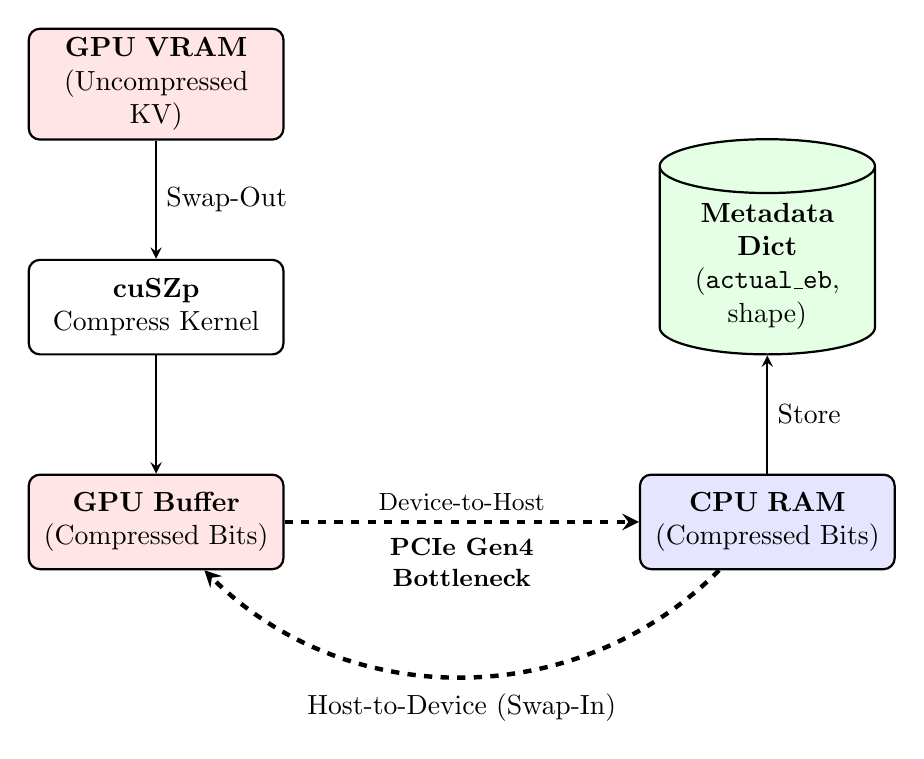
\begin{tikzpicture}[
        node distance=1.5cm and 4.5cm, % 适当加宽横向距离，给文字留空间
        box/.style={rectangle, draw=black, thick, text width=3cm, align=center, minimum height=1.2cm, rounded corners},
        db/.style={cylinder, draw=black, thick, aspect=0.25, text width=2.5cm, align=center, minimum height=1.5cm, shape border rotate=90},
        arrow/.style={thick, ->, >=stealth}
    ]
    
    % --- Nodes ---
    \node[box, fill=red!10] (vram) {\textbf{GPU VRAM}\\(Uncompressed KV)};
    \node[box, below=of vram] (compress) {\textbf{cuSZp}\\Compress Kernel};
    \node[box, below=of compress, fill=red!10] (comp_gpu) {\textbf{GPU Buffer}\\(Compressed Bits)};
    
    % 直接定位 comp_cpu，不再需要中间的 pcie 节点
    \node[box, right=of comp_gpu, fill=blue!10] (comp_cpu) {\textbf{CPU RAM}\\(Compressed Bits)};
    \node[db, above=of comp_cpu, fill=green!10] (dict) {\textbf{Metadata Dict}\\(\texttt{actual\_eb}, shape)};
    
    % --- Edges ---
    \draw[arrow] (vram) -- node[right] {Swap-Out} (compress);
    \draw[arrow] (compress) -- (comp_gpu);
    
    % 关键修改：一条线上放两个 node，一个在上一部在下
    \draw[arrow, dashed, ultra thick] (comp_gpu) -- 
        node[midway, above, font=\small] {Device-to-Host} 
        node[midway, below, yshift=-2pt, align=center, font=\bfseries\small] {PCIe Gen4\\Bottleneck} 
        (comp_cpu);
    
    \draw[arrow] (comp_cpu) -- node[right] {Store} (dict);
    
    % 下方的弧线
    \draw[arrow, dashed, ultra thick] (comp_cpu) to[bend left=45] 
        node[below, yshift=-2pt] {Host-to-Device (Swap-In)} (comp_gpu);
    
    \end{tikzpicture}
    \caption{Architectural flowchart of the \textbf{Compress-Transfer-Decompress} method. A large number of original kV tensors are compressed on the local GPU, and the minimized bit stream is transmitted with PCIe. The critical reconstruction metadata will be saved in the host RAM dictionary.}
    \label{fig:pipeline_diagram}
\end{figure}

\begin{itemize}
    \item \textbf{\texttt{compressed\_swap.py}:} This script connects vLLM to the compiled C++ backend. It defines a \texttt{CuSZpCompressor} class to configure the C++ wrapper with necessary error limits, \texttt{DIM\_1D} formatting, and GPU device mapping. The script also contains the \path{CompressedCacheEngineMonkeyPatch} class. When vLLM initializes, this patch class will automatically override the engine's default \texttt{\_swap\_out\_blocks\_to\_host} and \texttt{\_swap\_in\_blocks\_from\_host} methods. 
    
    For swap-out operations, the new function passes the raw GPU cache block to the compressor. The code then slices the resulting byte stream to remove the unused buffer and sends the exact payload to the CPU only, which significantly reduces transmission time. It records the compressed data and necessary reconstruction metadata, such as layer indices, tensor shape, and the specific \texttt{actual\_eb}, directly into the \texttt{compressed\_blocks\_store} dictionary. 
    
    For swap-in operations, the system retrieves the exact byte stream using its dictionary key and pushes it back to the GPU asynchronously via \path{tensor.cuda(non\_blocking=True)}. Finally, the decompressor reconstructs the data to exactly restore the vLLM cache block.

    \item \textbf{\texttt{test\_vllm\_integration.py}:} This script serves as a standalone unit test to verify the Monkey-Patching mechanism before running actual language models. The code sets up a \texttt{MockCacheEngine} to simulate vLLM's internal KV cache structure. It fills this mock cache with pseudo-random numbers and enforces the swap cycle. This test not only verifies that the Python hooks successfully intercept the memory routines but also confirms that the decompressed tensors match the original tensors within the allowable error bound.
\end{itemize}

\subsection{Integration and Infrastructure Deployment (\texttt{docker})}
\label{subsec:docker_deployment}

Managing dependencies like specific PyTorch versions, the CUDA toolkit, and the CMake compiler across different platforms (such as  Linux and Windows WSL2) often leads to environment conflicts. To ensure multi-platform stability, the system isolates the entire execution environment in the Docker container.

\begin{itemize}
    \item \textbf{\texttt{Dockerfile}:} The build starts from the \path{nvidia/cuda:12.1.1-devel-ubuntu22.04} base image to secure access to the NVCC compiler. The script will then install Python 3.10, essential system tools, and required pip packages. Instead of relying on pre-compiled binary files, the Dockerfile pulls the \texttt{cuSZp} source code directly from GitHub and compiles it globally. It then exports the required `LD\_LIBRARY\_PATH` so the custom PyBind11 wrapper can locate the CUDA libraries at runtime without triggering linking errors.
    
    \item \textbf{\texttt{run.sh}:} Manually typing a long Docker command is cumbersome and error-prone, so a dedicated shell script will manage the container lifecycle. It automatically fixes common Windows-to-Linux line-ending bugs (converting CRLF to LF) before execution. The script provides simple arguments to construct the image (\texttt{build}), open an interactive shell with GPU access (\texttt{run}), or execute the full benchmark script (\texttt{test}). This setup keeps the host machine completely clean while allowing users to trigger the entire pipeline using a single terminal command.
\end{itemize}


\section{Evaluation and Benchmarks}
\label{sec:evaluation_benchmarks}

\subsection{Experimental Setup}
The hardware baseline for these tests is a personal workstation equipped with an NVIDIA RTX 5080 GPU. This specific computation card utilizes high-bandwidth PCIe lanes, establishing a solid foundation for standard CPU-GPU data transmission speeds. 

The software environment runs on Linux and relies on PyTorch, vLLM, and the HuggingFace Transformers \cite{wolf-etal-2020-transformers} library. To prevent library version conflicts and ensure the tests are reproducible on other machines, Docker and the NVIDIA Container Toolkit have isolated the entire software stack, including the custom PyBind11 wrapper and CMake build tools.

\subsection{Benchmarking Pipeline}
Using random floating-point noise to test memory bandwidth can not accurately reflect the behavior of LLMs in production. Therefore, a custom Python script (\path{benchmark_pipeline.py}) was built to capture and test true LLM cache states.

\subsubsection{Methodology}
The pipeline script loads eight distinct advanced LLMs. To force these models to generate realistic, long-context hidden states, the tokenizer repeatedly (30$\times$) injects a dense informational prompt ``\textit{The Hong Kong Polytechnic University (PolyU) is a public research university located in Hung Hom, Hong Kong. }''. 

During the text generation stage, the script intercepts the actual Layer-0 key embeddings (\path{past\_key\_values[0][0]}). It flattens these multi-dimensional arrays and reshapes them to $4,194,304$ elements (approximately 16 MB in FP32). This step normalizes the memory footprint across all models while completely preserving the numerical distribution and local extreme values of tokens.

To record accurate timestamps without being affected by asynchronous GPU scheduling delays, the script places \texttt{torch.cuda.synchronize()} barriers around the host clock (\path{time.perf\_counter()}). Before recording any data, the system runs a mandatory warm-up stage: 10 dummy transfers for the uncompressed baseline, and 5 preliminary compression cycles to allocate all necessary VRAM pages. The script then executes 50 active iterations and averages the results to determine the final compression time, decompression latency, and effective bandwidth.

\subsubsection{Metrics}
The automated script tracks three main metrics:
\begin{itemize}
    \item \textbf{Compression Ratio}: The original tensor byte size divided by the size of the final compressed byte stream.
    \item \textbf{Absolute Max Error}: The mathematical difference between the original numbers and the decompressed numbers, ensuring it stays within the target bound of $\epsilon = 1 \times 10^{-4}$.
    \item \textbf{Baseline vs. Effective Bandwidth}: A comparison between the physical PCIe transfer speed (uncompressed) and the new effective transfer speed, which considers both the reduced payload size and the GPU compression/decompression time cost.
\end{itemize}

\subsection{Performance Results Analysis}
The script exports all execution logs into JSON files and compiles them as a Markdown summary. As Table \ref{tab:benchmark_results} and Figure \ref{fig:bandwidth_bar_chart} indicate, applying lossy compression to real KV cache tensors can obtain a performance gain.

In the architecture of the entire test, the pipeline reduces the physical data payload by 2.42$\times$ to 3.06$\times$. The maximum absolute error remains safely around the $10^{-3}$. By significantly reducing the size of the physical payload, the time saved on the PCIe bus can exceed the millisecond overhead of executing the cuSZp core on the GPU.

The Qwen2.5-1.5B model showed the highest single gain, hitting a 2.08$\times$ speedup for Swap-In operations. This effectively doubled the bandwidth from 16.32 GB/s to 33.86 GB/s. Other architectures like GPT-2, OPT, and Pythia have achieved extremely high speedup, which proves that the memory wall can be reliably bypassed by using the structural redundancy in the KV cache.

\begin{table}[htbp]
    \centering
    \caption{Compression Metrics and Effective Bandwidths vs. Uncompressed Baseline}
    \label{tab:benchmark_results}
    \resizebox{\textwidth}{!}{
    \begin{tabular}{l c c c c c c c c}
        \toprule
        \textbf{Model} & \textbf{Comp.} & \textbf{Max} & \textbf{Base} & \textbf{Effective} & \textbf{Out} & \textbf{Base} & \textbf{Effective} & \textbf{In} \\
        & \textbf{Ratio} & \textbf{Error} & \textbf{Swap-Out} & \textbf{Swap-Out} & \textbf{Speedup} & \textbf{Swap-In} & \textbf{Swap-In} & \textbf{Speedup} \\
        \midrule
        \textbf{GPT-2 (124M)} & 2.69$\times$ & $2.06 \times 10^{-3}$ & 8.25 GB/s & \textbf{14.60 GB/s} & \textbf{1.77$\times$} & 17.16 GB/s & \textbf{32.48 GB/s} & \textbf{1.89$\times$} \\
        \textbf{Qwen2.5-0.5B} & 2.42$\times$ & $2.52 \times 10^{-2}$ & 14.29 GB/s & \textbf{19.53 GB/s} & \textbf{1.37$\times$} & 17.92 GB/s & \textbf{30.52 GB/s} & \textbf{1.70$\times$} \\
        \textbf{Qwen2.5-1.5B} & 3.06$\times$ & $6.08 \times 10^{-2}$ & 14.56 GB/s & \textbf{22.24 GB/s} & \textbf{1.53$\times$} & 16.32 GB/s & \textbf{33.86 GB/s} & \textbf{2.08$\times$} \\
        \textbf{OPT-125M} & 2.63$\times$ & $1.27 \times 10^{-3}$ & 15.05 GB/s & \textbf{21.61 GB/s} & \textbf{1.44$\times$} & 20.75 GB/s & \textbf{37.36 GB/s} & \textbf{1.80$\times$} \\
        \textbf{OPT-350M} & 2.68$\times$ & $3.17 \times 10^{-4}$ & 12.33 GB/s & \textbf{18.60 GB/s} & \textbf{1.51$\times$} & 16.52 GB/s & \textbf{31.00 GB/s} & \textbf{1.88$\times$} \\
        \textbf{Pythia-160M} & 2.69$\times$ & $2.83 \times 10^{-3}$ & 13.20 GB/s & \textbf{19.77 GB/s} & \textbf{1.50$\times$} & 16.63 GB/s & \textbf{32.25 GB/s} & \textbf{1.94$\times$} \\
        \textbf{Pythia-410M} & 2.79$\times$ & $2.56 \times 10^{-3}$ & 14.41 GB/s & \textbf{21.78 GB/s} & \textbf{1.51$\times$} & 18.38 GB/s & \textbf{35.41 GB/s} & \textbf{1.93$\times$} \\
        \textbf{TinyLlama-1.1B} & 2.85$\times$ & $2.04 \times 10^{-3}$ & 14.29 GB/s & \textbf{21.69 GB/s} & \textbf{1.52$\times$} & 18.93 GB/s & \textbf{36.11 GB/s} & \textbf{1.91$\times$} \\
        \bottomrule
    \end{tabular}
    }
\end{table}

\begin{figure}[htbp]
    \centering
    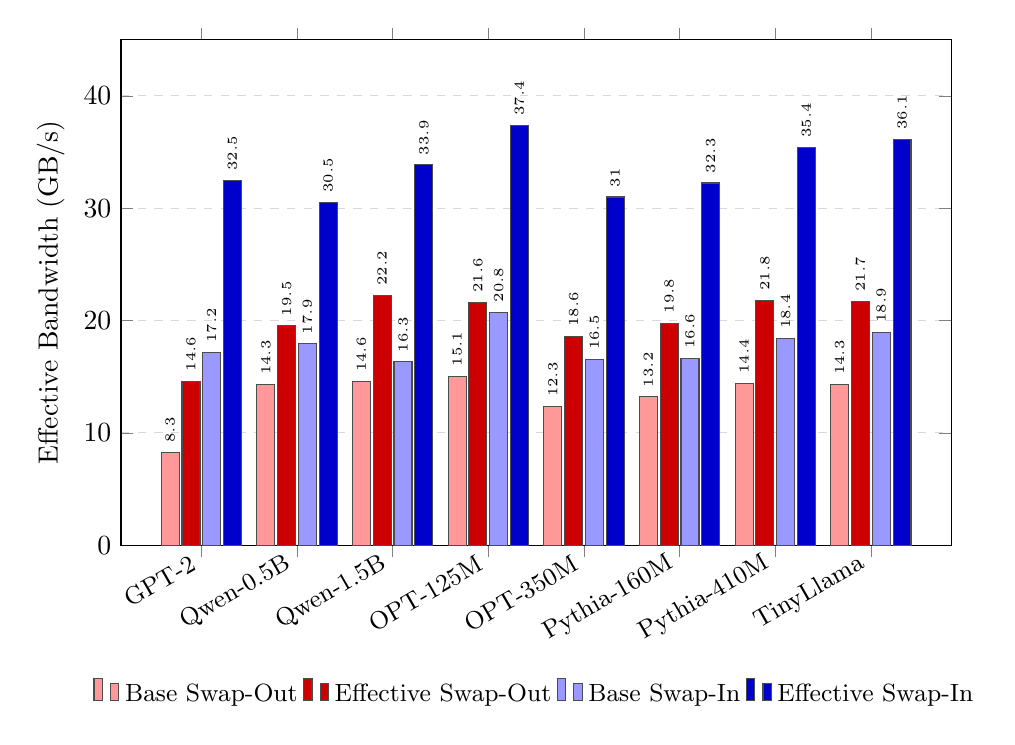
\begin{tikzpicture}
        \begin{axis}[
            ybar=1pt, % 柱子之间的间距缩小
            bar width=6.5pt, % 柱子调细，容纳4根
            width=\textwidth,
            height=8cm, % 稍微加高一点，给竖排数字留出空间
            enlarge x limits=0.12,
            legend style={at={(0.5,-0.25)}, anchor=north, legend columns=-1, draw=none, font=\small},
            ylabel={Effective Bandwidth (GB/s)},
            symbolic x coords={GPT-2, Qwen-0.5B, Qwen-1.5B, OPT-125M, OPT-350M, Pythia-160M, Pythia-410M, TinyLlama},
            xtick=data,
            x tick label style={rotate=30, anchor=east, font=\small},
            nodes near coords,
            % 将数字旋转90度，避免4个柱子的数字重叠
            every node near coord/.append style={font=\fontsize{5}{6}\selectfont, rotate=90, anchor=west, /pgf/number format/fixed, /pgf/number format/precision=1},
            ymin=0, ymax=45,
            ymajorgrids=true,
            grid style={dashed, gray!30}
        ]
        
        % 1. Base Swap-Out (浅红色)
        \addplot[fill=red!40, draw=black!70] coordinates {
            (GPT-2,8.25) (Qwen-0.5B,14.29) (Qwen-1.5B,14.56) 
            (OPT-125M,15.05) (OPT-350M,12.33) (Pythia-160M,13.20) 
            (Pythia-410M,14.41) (TinyLlama,14.29)
        };
        
        % 2. Effective Swap-Out (深红色)
        \addplot[fill=red!80!black, draw=black!70] coordinates {
            (GPT-2,14.60) (Qwen-0.5B,19.53) (Qwen-1.5B,22.24) 
            (OPT-125M,21.61) (OPT-350M,18.60) (Pythia-160M,19.77) 
            (Pythia-410M,21.78) (TinyLlama,21.69)
        };

        % 3. Base Swap-In (浅蓝色)
        \addplot[fill=blue!40, draw=black!70] coordinates {
            (GPT-2,17.16) (Qwen-0.5B,17.92) (Qwen-1.5B,16.32) 
            (OPT-125M,20.75) (OPT-350M,16.52) (Pythia-160M,16.63) 
            (Pythia-410M,18.38) (TinyLlama,18.93)
        };
        
        % 4. Effective Swap-In (深蓝色)
        \addplot[fill=blue!80!black, draw=black!70] coordinates {
            (GPT-2,32.48) (Qwen-0.5B,30.52) (Qwen-1.5B,33.86) 
            (OPT-125M,37.36) (OPT-350M,31.00) (Pythia-160M,32.25) 
            (Pythia-410M,35.41) (TinyLlama,36.11)
        };
        
        \legend{Base Swap-Out, Effective Swap-Out, Base Swap-In, Effective Swap-In}
        \end{axis}
    \end{tikzpicture}
    \caption{Comparison of Swap-Out and Swap-In Bandwidth across different LLMs. The cuSZp compression pipeline provides substantial improvements in effective data transmission rates over the uncompressed baseline for both bidirectional PCIe operations.}
    \label{fig:bandwidth_bar_chart}
\end{figure}

\subsection{Sensitivity Analysis of Error Bounds}
\label{subsec:sensitivity_analysis}

To map the exact trade-offs between tensor error and hardware speed, the script ran a sensitivity test on the GPT-2 and Qwen2.5 models. The relative error bound ($\epsilon_{rel}$) was incrementally moved from $10^{-2}$ to $10^{-5}$. The resulting latencies and ratios are recorded in Table \ref{tab:sensitivity_gpt2} and Table \ref{tab:sensitivity_qwen}.

% --- Table 2: GPT-2 ---
\begin{table}[htbp]
    \centering
    \small 
    \setlength{\tabcolsep}{3pt} 
    \caption{Impact of Relative Error Bounds on GPT-2 KV Tensor Compression (16 MB Original Size)}
    \label{tab:sensitivity_gpt2}
    \begin{tabularx}{\textwidth}{>{\hsize=1.2\hsize}Y >{\hsize=0.95\hsize}Y >{\hsize=0.95\hsize}Y >{\hsize=0.95\hsize}Y >{\hsize=0.95\hsize}Y}
        \toprule
        \textbf{Rel. Error Bound} ($\epsilon_{rel}$) & \textbf{Comp. Ratio} & \textbf{Max Abs Error} & \textbf{Comp. Time (ms)} & \textbf{Decomp. Time (ms)} \\
        \midrule
        $1 \times 10^{-2}$ & 6.02$\times$ & $2.06 \times 10^{-1}$ & 0.74 & 0.47 \\
        $1 \times 10^{-3}$ & 3.75$\times$ & $2.06 \times 10^{-2}$ & 0.78 & 0.51 \\
        \rowcolor{gray!10}
        $\mathbf{1 \times 10^{-4}}$ \textbf{(Def.)} & \textbf{2.69$\times$} & $\mathbf{2.06 \times 10^{-3}}$ & \textbf{0.76} & \textbf{0.50} \\
        $1 \times 10^{-5}$ & 2.10$\times$ & $2.06 \times 10^{-4}$ & 0.81 & 0.64 \\
        \bottomrule
    \end{tabularx}
\end{table}

% --- Table 3: Qwen2.5 ---
\begin{table}[htbp]
    \centering
    \small
    \setlength{\tabcolsep}{3pt}
    \caption{Impact of Relative Error Bounds on Qwen2.5-1.5B KV Tensor Compression (16 MB Original Size)}
    \label{tab:sensitivity_qwen}
    \begin{tabularx}{\textwidth}{>{\hsize=1.2\hsize}Y >{\hsize=0.95\hsize}Y >{\hsize=0.95\hsize}Y >{\hsize=0.95\hsize}Y >{\hsize=0.95\hsize}Y}
        \toprule
        \textbf{Rel. Error Bound} ($\epsilon_{rel}$) & \textbf{Comp. Ratio} & \textbf{Max Abs Error} & \textbf{Comp. Time (ms)} & \textbf{Decomp. Time (ms)} \\
        \midrule
        $1 \times 10^{-2}$ & 8.25$\times$ & $6.07 \times 10^{0}$ & 0.77 & 0.47 \\
        $1 \times 10^{-3}$ & 4.41$\times$ & $6.07 \times 10^{-1}$ & 0.87 & 0.60 \\
        \rowcolor{gray!10}
        $\mathbf{1 \times 10^{-4}}$ \textbf{(Def.)} & \textbf{3.06$\times$} & $\mathbf{6.08 \times 10^{-2}}$ & \textbf{0.81} & \textbf{0.55} \\
        $1 \times 10^{-5}$ & 2.30$\times$ & $6.08 \times 10^{-3}$ & 0.82 & 0.58 \\
        \bottomrule
    \end{tabularx}
\end{table}

\begin{figure}[htbp]
    \centering
    % --- 左图：GPT-2 ---
    \begin{minipage}{0.48\textwidth}
        \centering
        \resizebox{\linewidth}{!}{% <--- 强制缩放，绝对防溢出神器
        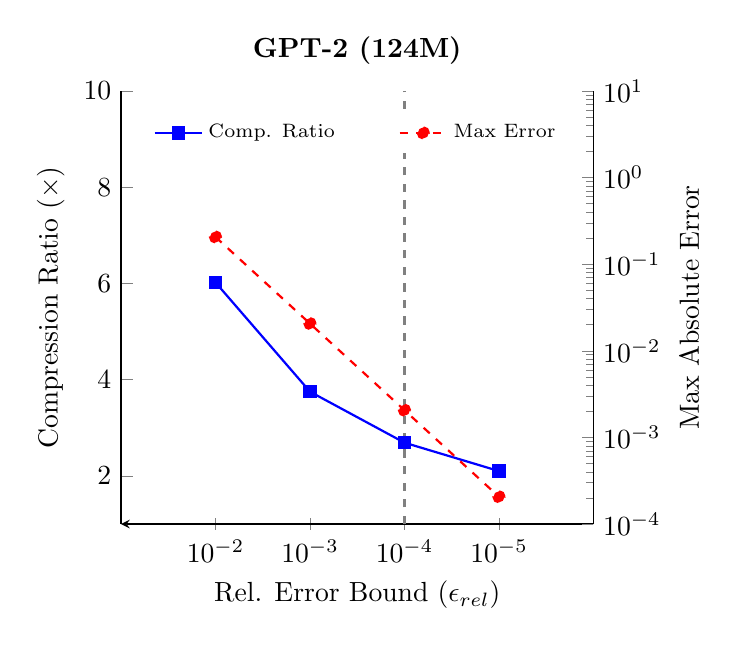
\begin{tikzpicture}
            % 左 Y 轴：压缩率
            \begin{axis}[
                title={\textbf{GPT-2 (124M)}},
                width=6cm,           % <--- 改为固定内部宽度
                height=5.5cm,        % <--- 改为固定内部高度
                scale only axis,
                xmode=log,
                x dir=reverse,
                xmin=1e-6, xmax=1e-1,
                xtick={1e-2, 1e-3, 1e-4, 1e-5},
                xlabel={Rel. Error Bound ($\epsilon_{rel}$)},
                ylabel={Compression Ratio ($\times$)},
                ymin=1, ymax=10,
                axis y line*=left,
                axis x line=bottom,
                legend style={at={(0.05,0.95)}, anchor=north west, draw=none, font=\fontsize{7}{8}\selectfont}
            ]
            \addplot[mark=square*, blue, thick] coordinates {
                (1e-2, 6.02)
                (1e-3, 3.75)
                (1e-4, 2.69)
                (1e-5, 2.10)
            };
            \addlegendentry{Comp. Ratio}
            
            \draw[dashed, gray, thick] (axis cs:1e-4, 1) -- (axis cs:1e-4, 10);
            \end{axis}

            % 右 Y 轴：最大绝对误差
            \begin{axis}[
                width=6cm,
                height=5.5cm,
                scale only axis,
                xmode=log,
                x dir=reverse,
                xmin=1e-6, xmax=1e-1,
                xtick=\empty,
                ylabel={Max Absolute Error},
                ymode=log,
                ymin=0.0001, ymax=10,
                axis y line*=right,
                axis x line=none,
                legend style={at={(0.95,0.95)}, anchor=north east, draw=none, font=\fontsize{7}{8}\selectfont}
            ]
            \addplot[mark=*, red, thick, dashed] coordinates {
                (1e-2, 0.206)
                (1e-3, 0.0206)
                (1e-4, 0.00206)
                (1e-5, 0.000206)
            };
            \addlegendentry{Max Error}
            \end{axis}
        \end{tikzpicture}
        }%
    \end{minipage}%
    \hfill
    % --- 右图：Qwen2.5 ---
    \begin{minipage}{0.48\textwidth}
        \centering
        \resizebox{\linewidth}{!}{% <--- 强制缩放，绝对防溢出神器
        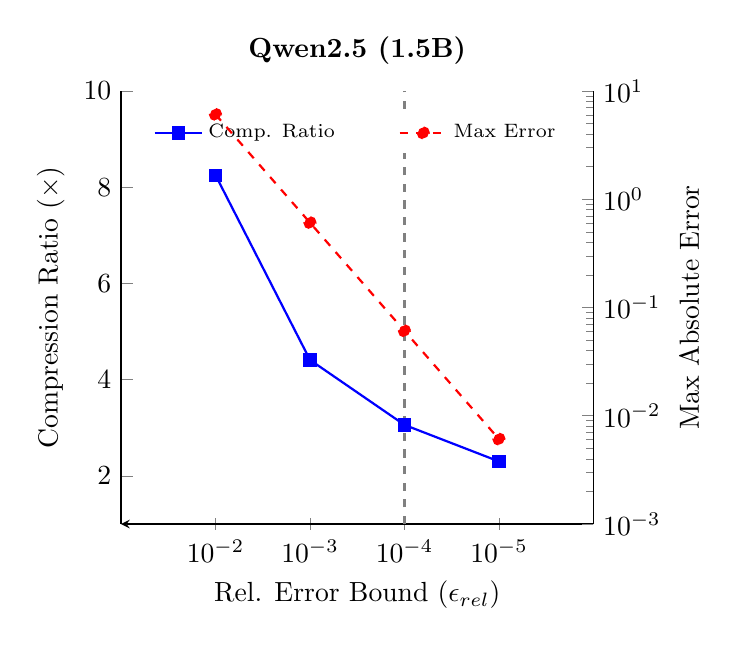
\begin{tikzpicture}
            % 左 Y 轴：压缩率
            \begin{axis}[
                title={\textbf{Qwen2.5 (1.5B)}},
                width=6cm,
                height=5.5cm,
                scale only axis,
                xmode=log,
                x dir=reverse,
                xmin=1e-6, xmax=1e-1,
                xtick={1e-2, 1e-3, 1e-4, 1e-5},
                xlabel={Rel. Error Bound ($\epsilon_{rel}$)},
                ylabel={Compression Ratio ($\times$)},
                ymin=1, ymax=10,
                axis y line*=left,
                axis x line=bottom,
                legend style={at={(0.05,0.95)}, anchor=north west, draw=none, font=\fontsize{7}{8}\selectfont}
            ]
            \addplot[mark=square*, blue, thick] coordinates {
                (1e-2, 8.25)
                (1e-3, 4.41)
                (1e-4, 3.06)
                (1e-5, 2.30)
            };
            \addlegendentry{Comp. Ratio}
            
            \draw[dashed, gray, thick] (axis cs:1e-4, 1) -- (axis cs:1e-4, 10);
            \end{axis}

            % 右 Y 轴：最大绝对误差
            \begin{axis}[
                width=6cm,
                height=5.5cm,
                scale only axis,
                xmode=log,
                x dir=reverse,
                xmin=1e-6, xmax=1e-1,
                xtick=\empty,
                ylabel={Max Absolute Error},
                ymode=log,
                ymin=0.001, ymax=10,
                axis y line*=right,
                axis x line=none,
                legend style={at={(0.95,0.95)}, anchor=north east, draw=none, font=\fontsize{7}{8}\selectfont}
            ]
            \addplot[mark=*, red, thick, dashed] coordinates {
                (1e-2, 6.07)
                (1e-3, 0.607)
                (1e-4, 0.0608)
                (1e-5, 0.00608)
            };
            \addlegendentry{Max Error}
            \end{axis}
        \end{tikzpicture}
        }%
    \end{minipage}
    \caption{Trade-off analysis between Compression Ratio (blue solid) and Max Absolute Error (red dashed) on GPT-2 and Qwen2.5 models. The vertical dashed lines denote the optimal selection boundary at $10^{-4}$ to ensure high bandwidth reduction while preventing destructive accuracy degradation.}
    \label{fig:sensitivity_line_chart}
\end{figure}

As documented in Table \ref{tab:sensitivity_gpt2}, Table \ref{tab:sensitivity_qwen}, and visualized in Figure \ref{fig:sensitivity_line_chart}, relaxing the error bound to $10^{-2}$ creates large compression ratios (6.02$\times$ for GPT-2 and 8.25$\times$ for Qwen2.5), significantly reducing the physical PCIe payload. However, this is at the cost of data corruption. At this loose boundary, the absolute error of Qwen2.5 is more than 6.0, and the error of GPT-2 reaches 0.2. In the context of transformer attention mechanisms, exponential Softmax operations seriously magnify these raw numerical deviations and completely destroy the quality of autoregressive generation of the model. On the contrary, forcing a tight bound of $10^{-5}$ can make the tensor almost the same as the original tensor, but the compression ratio will be reduced to about 2.10$\times$.

In addition, the logs always show that the execution time of the cuSZp compression kernel remains relatively stable (around 0.76 ms to 0.82 ms), regardless of how strict the error configuration is. This proves that on the RTX 5080, the bottleneck of the algorithm is simply the physical reading and writing to GPU VRAM, rather than the complexity of the internal mathematical branches. Based on these observations, $1 \times 10^{-4}$ is the optimal relative error bound across different model families. It can greatly reduce the payload size and provide effective bandwidth acceleration without damaging the internal state of the neural network.


\section{Discussion}
\label{sec:discussion}

\subsection{Interpretation of Results}

Benchmark logs reveal a significant gap in compression ratios between different architectures. For example, Qwen2.5-1.5B reached a 3.06$\times$ ratio, while 0.5B with a small parameter reached a peak of 2.42$\times$. This change can be attributed to the original data of the Key-Value (KV) cache tensors generated by each particular attention head. Naturally generated tensor models with a narrow range of values, high sparsity, or repetitive patterns will only give the cuSZp algorithm more space to compress data without breaking the strict absolute error limit.

The hardware configuration also proves that the NVIDIA RTX 5080 can reduce the algorithmic cost of the compression kernels. Powered by high-speed GDDR7 memory and modern multiprocessors, the GPU can execute the cuSZp routines in less than one millisecond. Due to the fast computation, the time saved by transmitting smaller payloads on the PCIe bus completely offsets the computational cost of compression. This raw hardware throughput is the main reason why the pipeline successfully provides end-to-end acceleration, such as the 2.08$\times$ improvement recorded during the tests.

\subsection{Implementation Challenges}

Building and deploying this compression pipeline exposed several low-level technical barriers, mainly involving PyTorch memory safety, parallel execution timing, and environment building.

\begin{itemize}
    \item \textbf{Memory Contiguousness:} Transferring data directly from Python to C++ requires strict memory layouts. After vLLM slicing or reshaping matrices for PagedAttention, the underlying PyTorch tensors are usually no longer stored in continuous memory blocks. If the C++ backend tries to read a fragmented tensor using the raw memory pointer, it will get data from the wrong physical address, which will immediately lead to data corruption and segmentation faults. To prevent this, the code calls \texttt{.contiguous()} on each target tensor, forcing the use of a unified memory layout before passing any pointers to the cuSZp kernels.
    
    \item \textbf{CUDA Stream Synchronization:} Managing PCIe transfers with active GPU computations is highly vulnerable to competitive conditions. Early iterations showed the CPU attempts to read memory before an asynchronous transfer finished, or start the decompressor before the byte stream completely reaches VRAM. To resolve this timing clash, the C++ wrapper pulls the active stream via \texttt{c10::cuda::getCurrentCUDAStream()}. This will force the custom cuSZp kernels to queue up safely in the native PyTorch execution process of vLLM, locking the operation order without pausing the GPU.
    
    \item \textbf{Cross-Platform Compilation:} Compiling the C++ codebase across different operating systems caused unexpected build failures. Moving project files between Windows (WSL2) and native Linux systems introduced hidden CRLF versus LF line-ending conflicts. These invisible returns completely broke the shell execution inside the Docker \texttt{run.sh} scripts and crashed the CMake configuration. The final deployment architecture includes automatic \texttt{sed} commands to clear these files before compilation, ensuring the container builds correctly regardless of the host machine.
\end{itemize}

\subsection{Limitations}

Although the transmission performance has been improved, the compression offload framework still has some noteworthy limitations:

\begin{itemize}
    \item \textbf{VRAM Overhead for Workspace Buffers:} A significant disadvantage is that running the cuSZp algorithm requires additional GPU VRAM. To prevent memory overflows, the compressor forces the system to allocate temporary workspace arrays and an oversized destination buffer for the unpredictable byte stream. Although the code frees this memory almost immediately after compression, the sudden spike in VRAM usage steals space from vLLM's active request pool. This creates a slight engineering paradox: the system must spend precious GPU memory momentarily just to execute the memory-saving offload operation.
    
    \item \textbf{Diminishing Returns on Small Batch Sizes:} The efficiency of the compressed pipeline is sensitive to the workload. In cases involving small batch sizes or extremely short context lengths, the absolute amount of KV cache being swapped is very small. In such cases, the fixed algorithm overhead caused by launching the CUDA compression kernel, combined with the baseline latency of initiating PCIe transfers, may completely offset the time savings achieved by transferring less data. Therefore, this framework is most advantageous in memory-bound, high-throughput environments (e.g., massive concurrent serving or processing extremely long documents) rather than highly latency-sensitive, single-batch inference tasks.
\end{itemize}


\section{Conclusion and Future Work}
\label{sec:conclusion}

\subsection{Summary of Achievements}
This Final Year Project designed, implemented, and evaluated a proof-of-concept data pipeline, demonstrating that enabling cuSZp compression can effectively accelerate key-value (KV) cache swapping operations in the vLLM inference engine. By utilizing a high-performance PyBind11 wrapper and dynamic Python Monkey-Patching, the proposed system transparently intercepts vLLM's standard memory manager. It applies hardware-accelerated, error-bounded lossy compression to drastically reduce the physical data footprint transferred between GPU VRAM and CPU host memory. Large-scale automated benchmarking on eight of the most advanced LLM architectures confirmed that the computational overhead introduced by the cuSZp algorithm is more than offset by the reduction in PCIe transfer time. Finally, this pipeline produces effective bandwidth acceleration (up to $2.08\times$), which can strictly maintain the quality of generation while alleviating the hardware bottleneck.

\subsection{Final Remarks}
The benchmark results from this project confirm that error-bounded lossy compression is a highly practical memory optimization for modern LLM serving. As context windows grow larger, simply buying more VRAM or upgrading to faster PCIe channels is rapidly becoming too expensive for most deployments. Splicing a high-speed software compressor like cuSZp directly into the KV cache lifecycle offers a direct workaround for the hardware memory wall. This approach proves that large-scale LLMs \cite{10.1145/3706418} can run efficiently without a lot of hardware expansion.

\subsection{Future Directions}
Although the current monkey-patched pipeline successfully accelerates cache offloading, future development can push the performance limits through three specific optimizations:

\begin{itemize}
    \item \textbf{Adaptive Error Bound Tuning:} The system currently calculates absolute error bounds based on a fixed relative percentage. Future versions can analyze attention weights \cite{zhang2023h2oheavyhitteroracleefficient} or token semantics during runtime to determine how sensitive a specific layer is. Then the pipeline can apply active compression to robust layers while strictly protecting fragile layers, pushing the compression ratio higher without breaking the text generation logic.
    
    \item \textbf{Native vLLM Core Integration:} Using Python Monkey-Patching and PyBind11 bridges introduces a slight context-switching delay. Rewriting the compression logic directly into the official C++ code base of vLLM will eliminate this situation. Injecting cuSZp directly into the engine's \texttt{BlockSpaceManager} and native PagedAttention kernels will allow the system to allocate and track variable-length memory blocks natively.
    
    \item \textbf{Asynchronous Chunk Pipelining:} Memory scheduling may become more aggressive in the next step. Instead of processing an entire KV cache block at once, the system can split the blocks into smaller chunks \cite{10.1145/3458817.3476145}. This will enable a pipeline: while the CPU transfers chunk $N$ over the PCIe bus, the GPU compresses chunk $N+1$ at the same time. Running these operations synchronously will hide the compression delay and keep the hardware fully saturated.
\end{itemize}

\clearpage
\addcontentsline{toc}{section}{References}
\bibliographystyle{IEEEtran}
\bibliography{refs}

\end{document}
